\section{User Journey Diagram}

\begin{figure}[H]
    \centering
    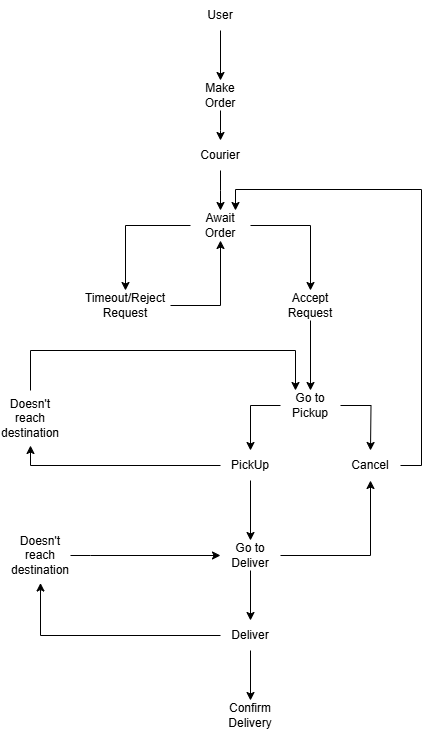
\includegraphics[width=0.6\textwidth]{images/UserJourney.png} % adjust path & width if needed
    \caption{Order journey diagram showing success and failure paths}
    \label{fig:user_journey}
\end{figure}

This diagram illustrates the typical order journey from a user's perspective, covering both successful and failed outcomes. It captures the interactions between clients, couriers, and the platform across different stages: order placement, courier acceptance, delivery progress, and resolution in case of errors or cancellations. The flow ensures that edge cases—such as order rejection or delivery failure—are considered during system design.

